\chapter{Higgs Analysis}
\label{Higgs Analysis}
Reinforce context for measurement as part of the higgs width measurement

Take everything from analysis note!!

lepton finding

jet finding- higgs and W mass plots

btagging

describe BDTs

final selection and uncertainty

Impact of this on the overall higgs measurements at CLIC \& compare to Higgs to qqqq channel

\section{Introduction}
One of the key aims for the CLIC experiment will be to perform a model independent measurement of the Higgs total width. Any deviations from the value predicted by the Standard Model for this would be clear evidence that there is new physics beyond the Standard Model involving particles that can interact with the Higgs. The size of any deviations could also give us an indication of the scale at which new physics occurs helping to guide the design of future high energy colliders. No current experiment has the capability of performing this measurement and so it is essential that is is measured at an electron-positron collider. The determination of the Higgs total width is dependent on the measurement of four quantities e.g. as described in Ref.\cite{Durig:2014lfa}. Here we will consider the measurement of one of these quanties, $\sigma_{H\nu\nu}$~x~Br$(H\rightarrow WW^*)$. As can be seen in Fig.\ref{fig:HiggsCrossSections}, this measurement is made possible during the 1.4TeV CLIC run as the cross section for the WW fusion process is the dominant Higgs production mechanism at this energy. This observable has already been studied at 1.4TeV using the WW$\rightarrow$qqqq channel \cite{Pandurovic:2011508}, yielding an expected statistical precision of 1.4\% for the nominal integrated luminosity of 1.5ab$^{-1}$. Here we will look at the complementary WW$\rightarrow$qql$\nu$ channel (shown in Fig.\ref{fig:feynmann}), where l=e,$\mu$, with the intention of combining our results with the existing measurement to estimate the overall precision acheivable at CLIC. 


\begin{figure}
  \centering
  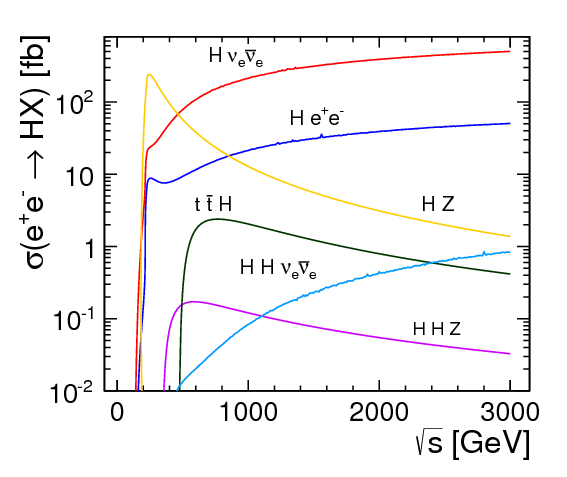
\includegraphics[width=0.48\textwidth,height=7cm,keepaspectratio]{/home/aw/github/thesis/HiggsAnalysis/figures/Midterm_HiggsCrossSections}
  \caption[Higgs Cross Sections]{Cross sections for Higgs production mechanisms in an ${e^+e^-}$ collider as a function of centre-of-mass energy \cite{Simon:2014aqa}. For energies above 500GeV, Higgs production is dominated by the WW-fusion process(red.)}
  \label{fig:HiggsCrossSections}
\end{figure}

\begin{figure}[h]
  \centering
  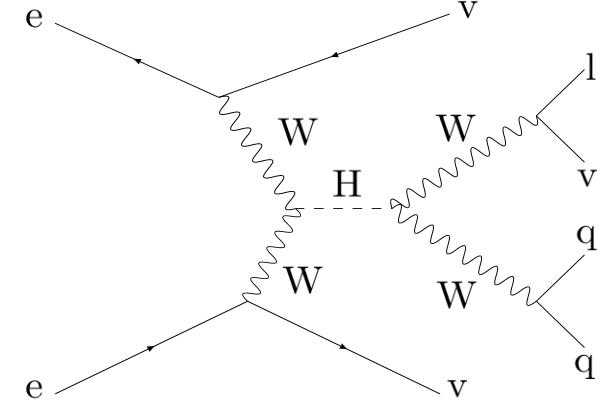
\includegraphics[width=0.48\textwidth,height=4.5cm,keepaspectratio]{/home/aw/github/thesis/HiggsAnalysis/figures/feynmann}
  \caption[Signal Feynmann Diagram]{Higgs production via WW fusion with the Higgs decaying to a WW pair, which then decays semileptonically.}
  \label{fig:feynmann}
\end{figure}


The signal and background processes we have examined in our analysis, along with their cross sections and sample production IDs, are summarised in Table. \ref{fig:backgrounds}. In all cases the detector model used is CLIC\_ILD\_CDR, a variant of the ILD detector designed for ILC \cite{CDR}. The main backgrounds of note are: the ee$\rightarrow$qql$\nu$ process (dominated by e$^+$e$^-\rightarrow$W$^+$W$^-$) as it has a very similar topology to our signal process and so is expected to be the most difficult to exclude; and the ee$\rightarrow$ H(WW$^*\rightarrow$qqqq)$\nu\nu$ process as our ability to correctly classify these events will determine how easily our results can be combined with measurements using this channel.

\renewcommand{\thefootnote}{\roman{footnote}}

\begin{figure}
  \centering
  \begin{tabular}{l r r r}
   \toprule
    Process     & Cross Section(fb)  &   Production ID\cite{bib-prodids}    & Events Used    \\
    \midrule
    Signal: ee$\rightarrow$ H(WW$^*\rightarrow$qql$\nu$)$\nu\nu$                & 18.9    &  2022\footnotemark[1]  & 70000  \\ 
    \midrule
    ee$\rightarrow$ H(WW$^*\rightarrow$qqqq)$\nu\nu$                & 25.6    &  2022\footnotemark[1]    & 140000 \\
    \midrule
    ee$\rightarrow$ H$^*\rightarrow$ Other & 199.6 & 2022\footnotemark[1] & 750000 \\
    \midrule
    ee$\rightarrow$qq               & 4009.5    &  2091  & 500000  \\ 
    \midrule
    ee$\rightarrow$qqqq               & 1328.1    &  2163  & 300000  \\ 
    \midrule
    e$\gamma$$\rightarrow$eqq ($\gamma$ from EPA)                 & 32308    &  2515\footnotemark[2] & 500000   \\ 
    \midrule
    $\gamma$e$\rightarrow$eqq ($\gamma$ from BS)               & 56043  &  2527\footnotemark[2]  & 500000 \\ 
    \midrule
    ee$\rightarrow$qq$\nu\nu$               & 787.7    &  3243 & 500000   \\ 
    \midrule
    ee$\rightarrow$qqll               & 2725.8    &  3246  & 400000  \\ 
    \midrule
    ee$\rightarrow$qql$\nu$              & 4309.7    &  3249 & 1000000   \\ 
    \bottomrule
  \end{tabular}
  \caption[Samples Used]{Samples used for the analysis}
  \label{fig:backgrounds}
\end{figure}

\footnotetext[1]{Sample 2022 is the ee$\rightarrow$H$\nu\nu$ inclusive sample. The relevant events were extracted from this main sample}
\footnotetext[2]{The cross-section for these events were scaled by a factor of 2 to account for interactions occuring with both the electron and positron. In the case of beamsstrahlung events simulated using GUINEA-PIG \cite{Schulte:382453}, a further scaling of 0.75 was applied to account for the lower luminosity of $e\gamma$ events} 

\section{Event Reconstruction}

Reconstruction of the signal events was performed using ILCSOFT v01-17-06 and was carried out in two main stages as described below. The first stage was to identify the isolated lepton associated with the leptonic W boson decay. The second stage involved removing this isolated lepton and resolving the remaining particles into two jets that were associated with the two quarks produced by the hadronically decaying W boson. Using the two jets, the W boson could then be reconstructed and combined with the isolated lepton to reconstruct the Higgs boson. The Higgs candidate we reconstruct will not be complete due to the lepton neutrino produced from the W decay. However, the observed properties will still be sufficient for discriminating between signal and background events.

\subsection{Lepton Identification}
Two different methods were used for identifying leptons. Our primary method for particle identification is to assume that the highest energy electron or muon (as identified by PandoraPFA \cite{Thomson200925}) corresponds to the isolated lepton from the leptonically decaying W boson. This method was found to have an efficiency and purity of 93\% and 96\% for identifiying the isolated lepton. 

The second method used a series of cuts to select the isolated lepton. The first stage of this was to group the particles in the event into four jets. This was done using FastJet \cite{Cacciari:2011ma} to implement the kt-algorithm using the E-scheme for recombination with an R-parameter of 0.4. We then required that the energy of the isolated lepton (electron or muon) constituted more than 35\% of the visible energy of the jet it was contained within. For electrons it was then required that at least 90\% of the total energy of the particle was deposited in the ECAL, and the ratio of energy to momentum for the particle was between 0.75 and 1.25. For muons it was required that less than 35\% of the total energy of the particle was deposited in the ECAL, and the ratio of energy to momentum should be between 0.01 and 0.60. This method yielded an efficiency of 91\% and a purity 74\%. Although this approach is not as performant as the first method, it allows more than one lepton to be selected. As a result it is useful for discriminating between signal and background processes as requirements can be placed on the number of leptons identified by this selection.

In summary, the first method is used to select a single isolated lepton, which is then used for reconstruction, while the number of lepton candidates selected by the second method is used as a discriminating variable to distinguish between signal and background processes. 

\subsection{Jet Finding}

Following the lepton finding, the remaining particles (not including the isolated lepton) are forced into two jets to reconstruct the properties of the two quarks produced from the hadronic W decay. This was carried out using the same jet finding algorithm as was used for the lepton identification. The optimization of the R-parameter was performed by using Monte Carlo information to obtain what mass we would measure for the reconstructed Higgs for various values of R, when using Monte Carlo truth kinematic information of the lepton neutrino in our reconstruction. An acceptably small bias in the reconstructed mass was found for an R value of 0.4, indicating we were successfully reconstructing the quark pair.

\section{Flavour Tagging}

\begin{figure}[b]
  \centering
  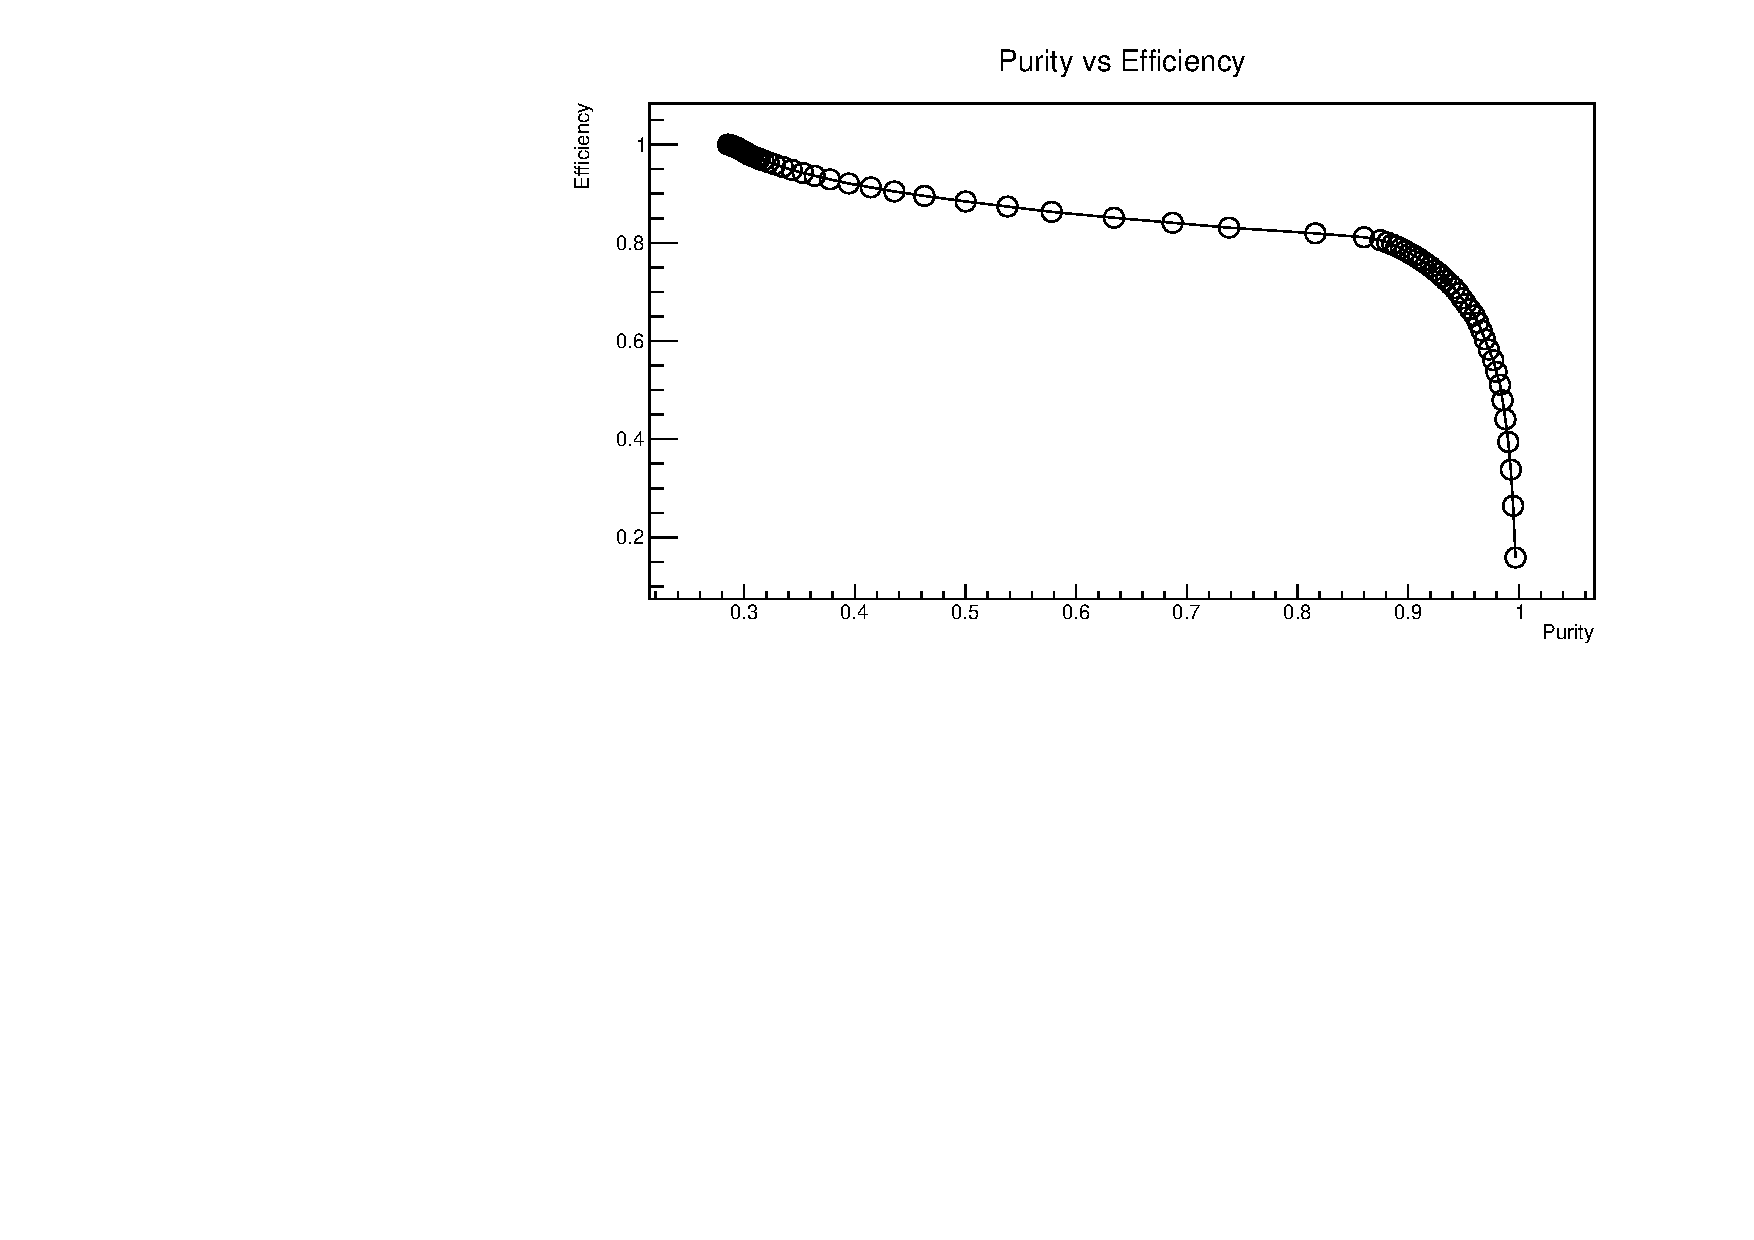
\includegraphics[width=0.78\textwidth,height=7cm,keepaspectratio]{HiggsAnalysis/figures/btag_crosses}
  \caption[B-Tagging Purity vs Efficiency]{Purity vs efficiency for identifying b-jets, obtained from a sample of Z$\rightarrow$ light, c and b quark events simulated at $\sqrt{s}=$1.4TeV}
  \label{btag}
\end{figure}

Flavour tagging of events was performed using LCFIPlus v00-05-02 \cite{Suehara:2015ura}. Three neural nets were trained to identify u/d/s, b and c quarks respectively with 50,000 ee$\rightarrow$ Z$\nu\nu$, Z$\rightarrow$qq events used for each neural net. Application of these neural nets returned two parameters for jets within the event that quantify the probability of the jet being either a b-jet or c-jet. For this analysis, identifying b-jets is more useful for discriminating against the relevant backgrounds. Performance of the b-tagging was evaluated by applying the neural nets to a sample of 150,000 events containing an equal number of Z$\rightarrow$ light, c and b quarks. It can be seen from Fig.\ref{btag} that a purity of 90\% can be achieved while still retaining an efficiency of 80\%.

\section{Event Selection}

Event selection was performed using the TMVA package \cite{2007physics...3039H} to produce a Boosted Decision Tree (BDT). The BDT used 7$\times$10$^4$ signal events and 4$\times$10$^6$ background events, split evenly between training and testing samples. A collection of 19 variables is used for the training: mass of the reconstructed Higgs and W bosons; energy of the W boson; missing energy and transverse momentum; number of isolated leptons selected; PID of lepton; transverse momentum of lepton; angle of lepton and W boson relative to the beam axis; magnitude of minor thrust value; number of particle flow objects (PFOs) in the two jets; average angle of the two jets relative to the beam axis; kt jet resolution parameter y$_{12}$; number of tightly selected PFOs in the event; angular separation of the isolated lepton and the W boson;  minimum angular separation and transverse momentum of the lepton relative to either jet, and the combined b-tag value for both jets. A set of loose pre-selection cuts were also applied before the training to remove events that were clearly background. The cuts used were: energy of the W boson <591GeV, Mass of the W boson <231GeV, Mass of the reconstructed Higgs <306GeV and 667GeV< total missing energy <1400GeV. The input signal and background distributions for every input variable after application of these cuts can be seen in the appendix, and the resulting BDT classifier output can be seen in Fig.\ref{bdt}.  

\begin{figure}
  \centering
  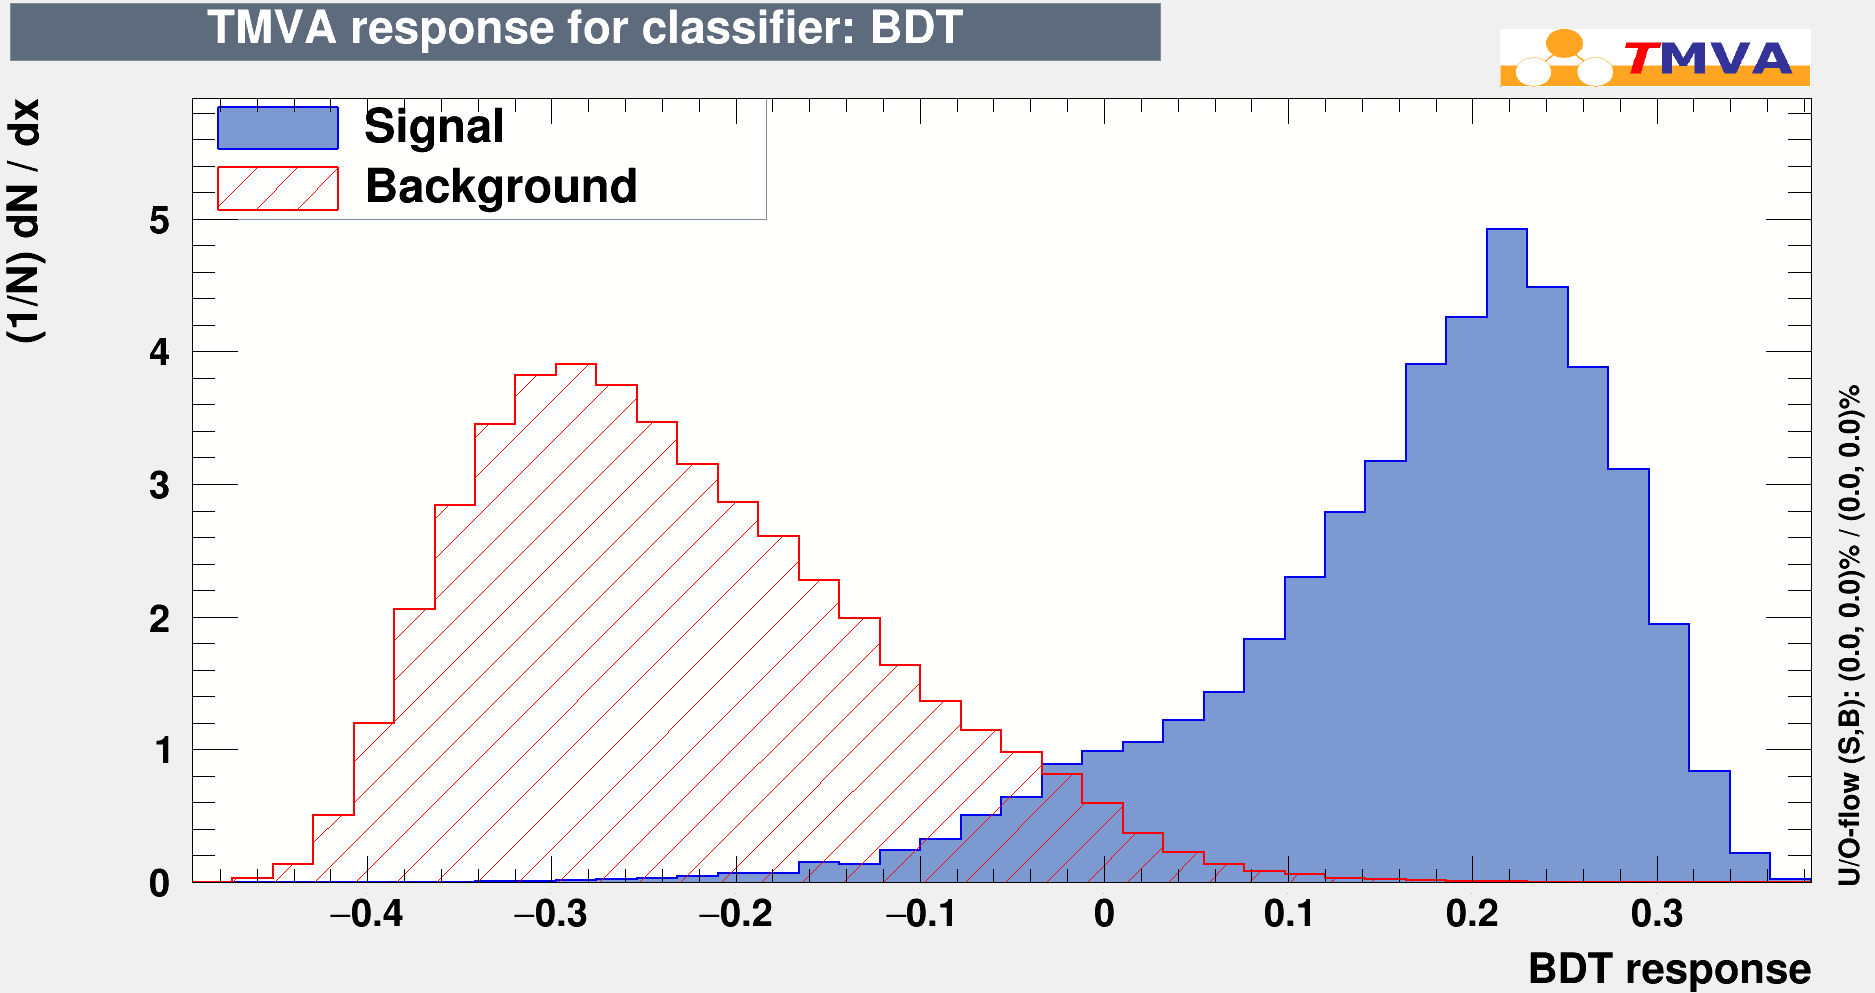
\includegraphics[width=0.68\textwidth,height=7cm,keepaspectratio]{/home/aw/github/thesis/HiggsAnalysis/figures/bdt}
  \caption[Classifier BDT response]{BDT response for signal and background events after TMVA classification}
  \label{bdt}
\end{figure}

Figure\ref{bdt} shows that there is a high degree of separation achieved between signal and background events. The optimal BDT cut for maximising the signal to background ratio was determined to be at 0.21 and the effect of the pre-selection cuts and applying this BDT cut on the signal and background processes can be seen in Fig. \ref{cuts}. The resulting significance ($S/\sqrt{S+B}$) after these cuts has been calculated to be 77 giving a statistical uncertainty of 1.3\% on $\sigma.$Br for an integrated luminosity of 1.5ab$^{-1}$. This value is similar to that observed for the WW$\rightarrow$qqqq final state, as expected. By neglecting the case where the isolated lepton it a $\tau$, we have reduced our statistics to two thirds that of the hadronic channel which inherently limits the precision that can be acheived. However, the backgrounds for the hadronic channel are much larger, making them harder to remove which leads to a reduced precision. Looking in detail at the backgrounds after our selection, we can see that many of the backgrounds have been almost completely removed leaving only ee$\rightarrow$ H($\rightarrow$ other)$\nu\nu$ and ee$\rightarrow$qql$\nu$ as the dominant backgrounds. This is to be expected as these events most closely mimic our signal, which is mainly distinguished by its large missing energy. In the case of H$\rightarrow$other events it was determined that 26\% of the remaining events came from H$\rightarrow\tau^+\tau^-$ processes with a further 25\% from H$\rightarrow$WW* processes with one or more of the Ws decaying to a $\tau$. As such, attempts were made to veto $\tau$ events by rejecting events in which one or more hadronically decaying $\tau$ was explicitly identified using a Tau Finder \cite{TauFinder}. However, the number of $\tau$s misidentified in the signal channel was determined to be too high to veto the $\tau$ events without significantly increasing the overall statisitcal uncertainty on $\sigma.$Br and so $\tau$ identification is not used in the final selection.
The efficiency for selecting WW$^*\rightarrow$qqqq events in the WW$^*\rightarrow$qql$\nu$ channel has been calculated to be 1.8\% which should be sufficiently low that a straightforward combination of the uncertainties determined by both channels can be made. However, further investigation must be done to confirm this. The efficiency of the H$\rightarrow$WW$\rightarrow$qql$\nu$ events in the H$\rightarrow$WW$\rightarrow$qqqq channel has yet to be confirmed, therefore a final combined result has not yet been performed. Where H$\rightarrow$WW candidates are identified by both selections, attributing them to a final state on the basis of the predicted purities, would simplify the calculation. Systematic uncertainties have not been described here but are expected to be dominated by the uncertainty on the measured WW$\rightarrow$qql$\nu$ branching ratio of 1.1\% \cite{Agashe:2014kda}. 

\begin{figure}
  \centering
  \begin{tabular}{l r r r r}
   \toprule
    Process & Cross Section(fb) & Pre-selection Eff(\%) & BDT Cut Eff(\%) & Events After BDT     \\
    \midrule
    Signal             & 18.9    &  99.99  & 42.65 & 12091    \\ 
    \midrule
    ee$\rightarrow$ H(WW$^*\rightarrow$qqqq)$\nu\nu$  & 25.6    &  99.96 & 1.79 & 687  \\
    \midrule
    ee$\rightarrow$ H($\rightarrow$ Other)$\nu\nu$ & 199.6 & 99.62 & 1.26 & 3767 \\
    \midrule
    ee$\rightarrow$qq               & 4009.5    & 76.95 &  <0.01 & 155  \\ 
    \midrule
    ee$\rightarrow$qqqq               & 1328.1    &  36.03 & <0.01 & 27   \\ 
    \midrule
    e$\gamma$$\rightarrow$eqq ($\gamma$ from EPA)                 & 32308    & 67.00  & <0.01 & 816    \\ 
    \midrule
    $\gamma$e$\rightarrow$eqq ($\gamma$ from BS)               &  56043   & 95.84 & <0.01 & 764  \\ 
    \midrule
    ee$\rightarrow$qq$\nu\nu$               & 787.7    & 96.59 & 0.07 & 777   \\ 
    \midrule
    ee$\rightarrow$qqll               & 2725.8    & 89.75  & <0.01 & 257    \\ 
    \midrule
    ee$\rightarrow$qql$\nu$              & 4309.7    & 66.44  & 0.07 & 4812    \\ 
    \bottomrule
  \end{tabular}
  \caption[Samples Used]{Efficiency for all processes following pre-selection and BDT response cuts and the number of events expected to satisfy these requirements, for an integrated luminosity of 1.5ab$^{-1}$.}
  \label{cuts}
\end{figure}

\section{Conclusion}

In summary, we have performed a full analysis of the ee$\rightarrow$ H(WW$^*$)$\nu\nu$, WW$^*\rightarrow$qql$\nu$ decay channel using a large set of backgrounds with the aim of measuring the H$\rightarrow$WW$^*$ branching ratio. A 19 variable BDT was used to select signal events where the final state charged lepton is either an electron or a muon, and to remove background which was found to be dominated by ee$\rightarrow$ H($\rightarrow$ Other)$\nu\nu$  and ee$\rightarrow$qql$\nu$ in the final selection. The resulting statistical uncertainty was found to be: \\[10pt]\centerline{\large{$\delta\sigma_{H\nu\nu}$ x BR(H$\rightarrow$WW$^*$) = 1.3\%}} \\[10pt] The efficiency for incorrectly selecting ee$\rightarrow$H(WW$^*$)$\nu\nu$, with WW$^*\rightarrow$qqqq, in the WW$^*\rightarrow$qql$\nu$ channel, was found to be 1.8\%. The correlated overlap in selections developed for the WW$^*\rightarrow$qqqq and WW$^*\rightarrow$qqlv final states would be taken into account when combining the individual results.
 
